% The one equation of the talk, thesis Eq. (eom): M(Y) qdd + C qd + K q = u with u = P u_act,
% each term labelled in words. Labels alternate above and below so they cannot collide.
\documentclass[border=8pt]{standalone}
% Shared preamble of the TikZ slide figures. Role colours match style.py.
\usepackage[T1]{fontenc}
\usepackage[scaled]{helvet}
\renewcommand\familydefault{\sfdefault}
\usepackage{amsmath}
\usepackage{tikz}
\usetikzlibrary{arrows.meta,calc,decorations.pathmorphing,positioning}
\definecolor{cbase}{HTML}{D55E00}   % physics model
\definecolor{caug}{HTML}{0072B2}    % augmented model, no projection
\definecolor{cproj}{HTML}{009E73}   % augmented model with projection
\definecolor{cink}{HTML}{222222}
\definecolor{cmuted}{HTML}{6B6B6B}

\begin{document}
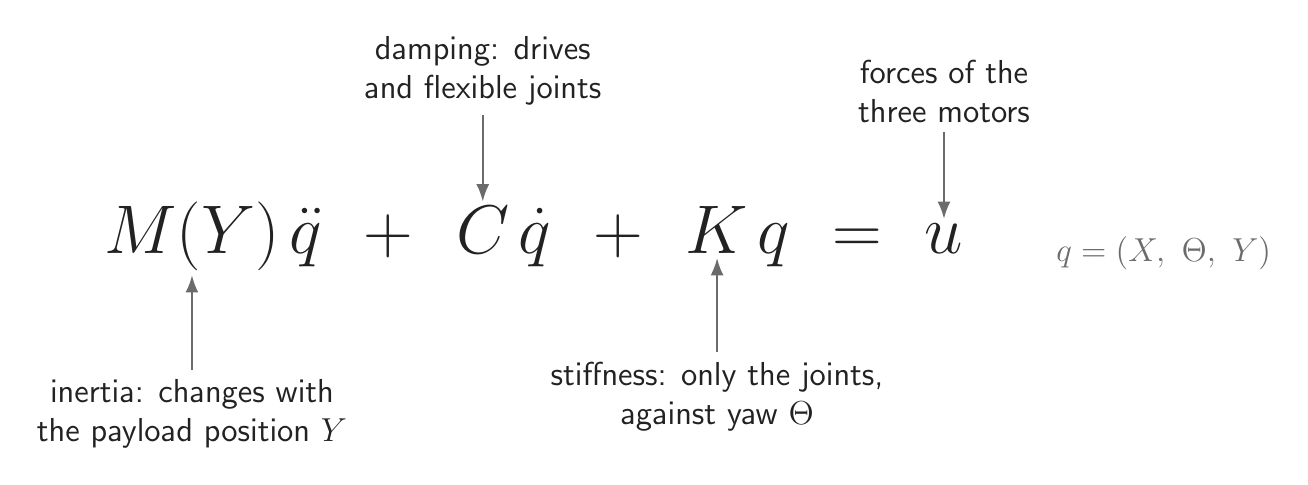
\begin{tikzpicture}[
    t/.style={inner sep=1.5pt, font=\Huge, text=cink},
    lab/.style={font=\large, align=center, text=cink},
    pt/.style={-{Latex[length=2.2mm]}, cmuted, line width=0.8pt}]
  \node[t] (M) {$M(Y)$};
  \node[t, base right=0pt of M] (qdd) {$\ddot q$};
  \node[t, base right=12pt of qdd] (p1) {$+$};
  \node[t, base right=12pt of p1] (C) {$C$};
  \node[t, base right=0pt of C] (qd) {$\dot q$};
  \node[t, base right=12pt of qd] (p2) {$+$};
  \node[t, base right=12pt of p2] (K) {$K$};
  \node[t, base right=0pt of K] (q) {$q$};
  \node[t, base right=12pt of q] (eq) {$=$};
  \node[t, base right=12pt of eq] (u) {$u$};

  \node[lab, below=12mm of M] (lM) {inertia: changes with\\the payload position $Y$};
  \node[lab, above=11mm of C] (lC) {damping: drives\\and flexible joints};
  \node[lab, below=12mm of K] (lK) {stiffness: only the joints,\\against yaw $\Theta$};
  \node[lab, above=11mm of u] (lu) {forces of the\\three motors};
  \draw[pt] (lM.north) -- (M.south);
  \draw[pt] (lC.south) -- (C.north);
  \draw[pt] (lK.north) -- (K.south);
  \draw[pt] (lu.south) -- (u.north);

  \node[font=\large, text=cmuted, anchor=west] at ($(u.base east)+(10mm,0)$)
       {$q = (X,\ \Theta,\ Y)$};
\end{tikzpicture}
\end{document}
